\ifx \allfiles \undefined
\documentclass[12pt,a4paper,oneside]{article}

%% === CJK 套件 ===
\usepackage{CJKutf8,CJKnumb}                 % 中文套件
%% === AMS 標準套件 ===
\usepackage{amsmath,amsfonts,amssymb,amsthm} % 數學符號
%% === ===
\usepackage{algorithm}
\usepackage{listings}                        % 程式碼
%% === TikZ 套件 ===
\usepackage{tikz,tkz-graph,tkz-berge}        % 繪圖
\usepackage{multicol}
%% == ==
\usepackage[unicode]{hyperref}
\usepackage{xcolor}
\hypersetup{
    colorlinks,
    linkcolor={blue!100!black},
    citecolor={blue!75!black},
    urlcolor={blue!50!black}
}
%% == 調整設定 ==
\usepackage{enumitem}                           % 修改 enumerate, item
\usepackage{bbding}
\usepackage{titletoc,titlesec,imakeidx}
%% == ==
\usepackage{newfloat}
\usepackage{caption,subcaption}
\usepackage{xkeyval,xargs}
\usepackage{ulem}
\usepackage{import}

%% === 設定 C++ 格式 ===
\lstset{%
  language=C++,             % 設定語言
  %% === 空白, tab 相關 ===
  tabsize=2,                % 設定 tab = 多少空白
  %showspaces=true,          % 設定是否標示空白
  %showtabs=true,            % 設定是否標示 tab
  %tab=\rightarrowfill,      % 設定 tab 樣式
  %% === 行數相關 ===
  numbers=left,             % 行數標示位置
  stepnumber=1,             % 每隔幾行標示行數
  numberstyle=\tiny,
  %breaklines=true,          % 設定斷行
  %% === 顏色設定 ===
  basicstyle=\ttfamily,
  keywordstyle=\color{blue}\ttfamily,
  stringstyle=\color{red!50!brown}\ttfamily,
  commentstyle=\color{green!50!black}\ttfamily,
  %identifierstyle=\color{black}\ttfamily,
  emphstyle=\color{purple}\ttfamily,
  extendedchars=false,
  texcl=true,
  moredelim=[l][\color{magenta}]{\#},
  captionpos=b,
  %% === 其他 ===
  %frame=single
}

% ===============================================
%
%  設定頁面格式
%
% ===============================================
%% === 設定頁面格式 ===
%\hoffset         = 10pt                      % 水平位移,預設為 0pt
\voffset         = -15pt                     % 垂直位移,預設為 0pt
\oddsidemargin   = 0pt                       % 預設為 31pt
%\topmargin       = 20pt                      % 預設為 20pt
%\headheight      = 12pt                      % header 的高度,預設為 12pt
%\headsep         = 25pt                      % header 和 body 的距離,預設為 25pt
\textheight      = 620pt                     % body 內文部分的高度,預設為 592pt
\textwidth       = 450pt                     % body 內文部分的寬度,預設為 390pt
%\marginparsep    = 10pt                      % margin note 和 body 的距離,預設為 10pt
%\marginparwidth  = 35pt                      % margin note 的寬度,預設為 35pt
%\footskip        = 30pt                      % footer 高度 + footer 和 body 的距離,預設為 30pt

%% ==  ==
\DeclareFloatingEnvironment[fileext=frm,placement={!ht},name=Frame]{code}
\captionsetup[code]{labelfont=bf}

\makeindex

\linespread{1.14}

\begin{document}
\begin{CJK}{UTF8}{bkai}

\subimport{./config/}{docsetting.tex}
\setcounter{section}{1}

\fi

\section{程式架構解析}

\paragraph{}這一節主要延續上一節的思維,但著重在了解程式如何執行,利用這些知識順利寫出\textbf{架構簡潔}、\textbf{容易除錯}程式。因此在這一節練習題較少,大多是\textbf{重要的觀念}。

\subsection{位址與指標}

\subsubsection{溢位現象}

\paragraph{}以下程式碼會發生什麼現象?
\begin{code}[h!]
\centering
\begin{tabular}{c}
\begin{lstlisting}
int x = 2147483647;
cout << x + 1 << endl;
\end{lstlisting}
\end{tabular}
\caption{產生溢位的程式碼}
\label{program:struct:code:overflow}
\end{code}

\paragraph{}若讀者的 \lstinline!int! 也是 4 個位元組的話,那麼就會得到 \lstinline!-2147483648!!這種現象我們稱為\index{溢位}{\textbf{溢位現象 (Overflow)}}。我們從二進位下看這段程式,會比較了解:

\begin{table}[h!]
\centering
\begin{tabular}{|c|c|c|c|}
\hline
$01111111$ & $11111111$ & $11111111$ & $11111111$\\
\hline
\end{tabular}
\caption{\lstinline!2147483647!}
\label{program:struct:table:binary:2147483647}
\end{table}

\paragraph{}表 \ref{program:struct:table:binary:2147483647} 表示 \lstinline!2147483647! 在 \texttt{C++} 當中如何儲存,讀者可以驗證 $2147483647=2^{31}-1$。若我們此時對 \lstinline!2147483647! 加 \lstinline!1!,就會得到下面的結果:

\begin{table}[h!]
\centering
\begin{tabular}{|c|c|c|c|}
\hline
${\color{red}1}0000000$ & $00000000$ & $00000000$ & $00000000$\\
\hline
\end{tabular}
\caption{\lstinline!2147483647 + 1!}
\end{table}

\paragraph{}我們用 \lstinline!int! 的儲存方法驗證,這個數字就是 \lstinline!-2147483648!,也就是 $-2^{32}$!為什麼會這樣子呢?
\paragraph{}我們可以建立一個有點抽象的概念,只要表示資料的\textbf{方法}所以用的記憶體大小是\textbf{有限}的,那麼就只能表示\textbf{有限多種}資料。例如:\lstinline!int! 通常是 4 個位元組,也就是 $4\times{8}=32$ 個位元,每個位元只能表示 \lstinline!0! 和 \lstinline!1! 兩種可能性,則最多只能表示 $2^{32}$ 種整數。
\paragraph{}這 $2^{32}$ 種整數表示法當中,我們切一半,$2^{31}$ 個表示負數,$2^{31}$ 表示非負整數,其中有一個 $0$,剩下 $2^{31}-1$ 個是正整數,因此 \lstinline!int! 的範圍就是介於 $-2^{31}$ 到 $2^{31}-1$。

\begin{table}[h!]
\centering
\begin{tabular}{|c|c|c|c|}
\hline
\textbf{資料型態} & \textbf{位元組} & \textbf{通常下界} & \textbf{通常上界}\\
\hline\hline
\lstinline!char!      & 1 & $-128$        & $127$       \\
\hline
\lstinline!short!     & 2 & $-32768$      & $32767$     \\
\hline
\lstinline!int!       & 4 & $-2147483648$ & $2147483647$\\
\hline
\lstinline!long long! & 8 & $-9223372036854775808$ & $9223372036854775807$\\
\hline
\lstinline!float!     & 4 & $-3.40282\times{10^{38}}$ & $3.40282\times{10^{38}}$\\
\hline
\lstinline!double!    & 8 & $-1.79769\times{10^{308}}$ & $1.79769\times{10^{308}}$\\
\hline
\lstinline!unsigned char!      & 1 & $0$ & $255$\\
\hline
\lstinline!unsigned short!     & 2 & $0$ & $65535$\\
\hline
\lstinline!unsigned int!       & 4 & $0$ & $4294967295$\\
\hline
\lstinline!unsigned long long! & 8 & $0$ & $18446744073709551615$\\
\hline
\end{tabular}
\caption{資料型態上下界}
\label{program:struct:table:datatype:limit}
\end{table}

\paragraph{}表 \ref{program:struct:table:datatype:limit} 表示每一種資料型態常見的上下界範圍,其中 \lstinline!unsigned! 類型代表「\textbf{不帶負號}」,也就是說 \lstinline!unsigned! 系列會把所有符號拿去表示非負整數。
\paragraph{}此外,需要注意的有幾點:
\begin{itemize}
\item \lstinline!int! 的上限是 \lstinline!2147483647!,用十六進位表示為 \lstinline!0x7FFFFFFF!
\item \lstinline!long long! 範圍大概是 $-9\times{10^{18}}$ 到 $9\times{10^{18}}$ 之間
\item \lstinline!double! 的範圍介於 $-{10}^{308}$ 至 ${10}^{308}$ 左右
\end{itemize}
\paragraph{}這些範圍可以在標頭檔 \index{climits}{\lstinline!<climits>!} 和 \index{cfloat}{\lstinline!<cfloat>!} 當中查詢到,實際範圍會依據不同計算機而有差異,使用方法自行 google,這裡不贅述。

\subsubsection{記憶體}

\paragraph{}之前我們提到\index{位元}{位元}和\index{位元組}{位元組}以及 \lstinline!sizeof! 等觀念,接下來要進入有關\index{記憶體}{\textbf{記憶體}}的部分。首先,我們常常提到的記憶體有分廣義和狹義的分別,廣義的記憶體可以指稱所有儲存資料的設備,表 \ref{program:struct:table:hierarchical:memory} 列出計算機中常用的儲存設備:

\begin{table}[h!]
\centering
\begin{tabular}{|c|c|c|c|c|}
\hline
\textbf{種類}                                          & \textbf{原文} & \textbf{存取速度} & \textbf{容量} & \textbf{用途}                                              \\
\hline\hline
\color{blue}\textbf{暫存器} & Register & 1 CPU  週期 & 數百 Bytes 內 & \begin{tabular}[c]{@{}c@{}}CPU 內部暫存\\ 運算的資料\end{tabular}   \\
\hline
快取記憶體 & Cache & 數十 CPU 週期 & 數十 MB 內 & \begin{tabular}[c]{@{}c@{}}協調 CPU 和\\ 主記憶體的速度\end{tabular} \\
\hline
\color{red}\textbf{主記憶體} & Main Memory & 數百 CPU 週期 & 8 GB 左右 & \begin{tabular}[c]{@{}c@{}}執行程式、\\ 暫存資料等\end{tabular}      \\
\hline
\color{blue}\textbf{\begin{tabular}[c]{@{}c@{}}碟盤設備\\ (硬碟、光碟)\end{tabular}} & Disk Storage & 數百萬 CPU 周期 & 數 TB          & \begin{tabular}[c]{@{}c@{}}永久儲存\\ 程式、資料\end{tabular}       \\
\hline
\end{tabular}
\caption{廣義的記憶體,又稱為\textbf{記憶體階層} (2016年資料)}
\label{program:struct:table:hierarchical:memory}
\end{table}

\paragraph{}狹義的記憶體就是\textbf{主記憶體},俗稱「\index{記憶體}{\textbf{記憶體}}」,程式在開始運行前,會將存在硬碟當中的程式資料移到記憶體當中,才會執行程式。

\subsubsection{位址}

\paragraph{}主記憶體可以看做是一條很長、連續的位元組,程式執行時,會佔據其中一個位置,如圖 \ref{program:struct:fig:memory:and:program}:

\begin{figure}[h!]
\centering
\begin{tikzpicture}
\edef\mywd{2}
\draw (0,0) rectangle (10,\mywd);
\filldraw[black!30!white,draw=black] (4,0) rectangle (6,\mywd) node[black,pos=0.5] {程式};
\node at (-1,.5*\mywd) {記憶體};
\end{tikzpicture}
\caption{記憶體與程式}
\label{program:struct:fig:memory:and:program}
\end{figure}

\paragraph{}記憶體可以比作「\textbf{土地}」,一開始有一大片未經使用的土地,由作業系統和程式去分配用途,為了方便管理記憶體,計算機會幫每個{\color{blue}\textbf{位元組}}標記「\textbf{地址}」,在此我們就稱為「\index{位址}{\color{red}\textbf{位址}}」。
\paragraph{}此外,位元組是擁有地址的{\color{blue}\textbf{最小單位}},單個位元並沒有位址。

\paragraph{取址運算子}位址通常是一個 16 進位的數字,如果我們要知道一個變數的位址,我們使用\index{取址運算子}{取址運算子} \lstinline!&!,例如程式碼 \ref{program:struct:code:address}:

\begin{code}[h!]
\centering
\begin{tabular}{c}
\begin{lstlisting}
int a = 16;
cout << "Address of a = " << &a << endl;
\end{lstlisting}
\end{tabular}
\caption{印出 \lstinline!a! 的位址}
\label{program:struct:code:address}
\end{code}

\paragraph{}筆者的執行結果為:\lstinline!Address of a = 003FF07C!,代表變數 \lstinline!a! 實際的位址是在 \lstinline!0x003FF07C! 的位元組,相當於是他的「\textbf{門牌號碼}」,因為 \lstinline!int! 通常為 4 個位元組,因此會佔據 \lstinline!0x003FF07C!、\lstinline!0x003FF07D!、\lstinline!0x003FF07E!、\lstinline!0x003FF07F! 這四個位元組。如圖 \ref{program:struct:fig:int:address}:

\begin{figure}[h!]
\centering
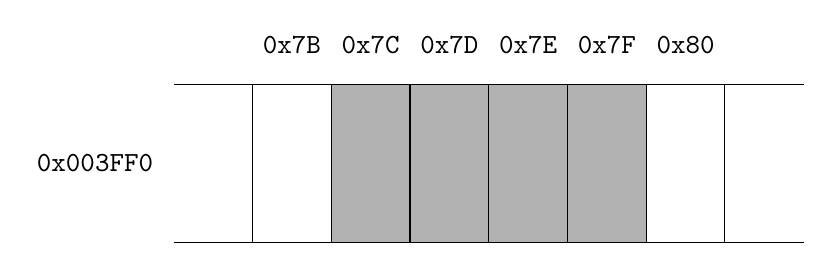
\begin{tikzpicture}
\def\arr{7B,7C,7D,7E,7F,80};
\draw (0,0) -- (8,0);
\draw (0,2) -- (8,2);
\edef\myleft{0}
\edef\myright{0}
\edef\mypos{0}
\foreach \item [count=\i] in \arr
{
	\ifthenelse{1<\i \AND \i<6}{%
		\fill[black!30!white] (\i,0) rectangle (\i+1,2);
	}{}
	\draw (\i,0) rectangle (\i+1,2);
	\node at (\i+0.5,2.5) {\texttt{0x\item}};
}
\node at (-1,1) {\texttt{0x003FF0}};
\end{tikzpicture}
\caption{變數 \lstinline!a! 實際的記憶體位置}
\label{program:struct:fig:int:address}
\end{figure}

\paragraph{}這個結果會因為不同機器、每次程式執行分配的記憶體不同而不一樣 (總之就是\textbf{不一定}啦!(╯°□°)╯︵ ╧╧),但概念是相同的。

\paragraph{大印第安和小印第安}但是我們要怎麼知道變數 \lstinline!a! 實際怎麼儲存在記憶體中呢?很多人會以為像是圖 \ref{program:struct:fig:big:endian}:

\begin{figure}[h!]
\centering
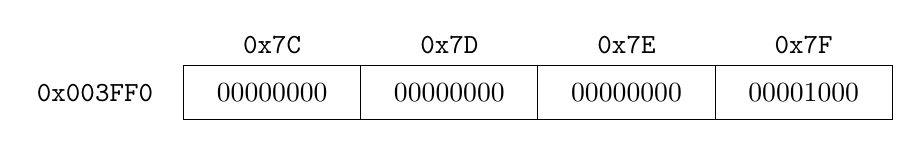
\begin{tikzpicture}
\def\sz{3mm}
\def\mywd{7.5}
\def\myht{2.3}
\tikzset{bit block/.style={
	draw,
	rectangle,
	minimum height=\myht*\sz,
	minimum width=\mywd*\sz
}}
\def\addr{7C,7D,7E,7F};
\def\arr{$00000000$,$00000000$,$00000000$,$00001000$};
\foreach \item [count=\i] in \arr
{
	\node[bit block] at (\i*\mywd*\sz,0) {\item};
}
\foreach \item [count=\i] in \addr
{
	\node at (\i*\mywd*\sz,.6) {\texttt{0x\item}};
}
\node at (0,0) {\texttt{0x003FF0}};
\end{tikzpicture}
\caption{大印地安儲存方法}
\label{program:struct:fig:big:endian}
\end{figure}

\subsubsection{指標}

\subsubsection{記憶體操作}

\subsection{執行時期配置}

\subsection{程式控制}

\subsubsection{程式區塊}

\subsubsection{分支結構}

\paragraph{應用:找極值}

\subsubsection{迴圈結構}
\subsubsection{陣列}

\subsection{函數}
\subsubsection{傳值呼叫}
\subsubsection{傳址呼叫}
\subsubsection{傳參考呼叫}
\subsubsection{函數多載}
\subsubsection{程式區塊}

\subsection{程式技巧}
\subsubsection{函式化}
\subsubsection{\lstinline!\#define! 與 \lstinline!inline!}

\subsection{\texttt{C++} 物件導向}
\subsubsection{物件與類別}
\subsubsection{建構子與解構子}
\subsubsection{運算子多載}

\ifx \allfiles \undefined

\printindex

\clearpage
\end{CJK}
\end{document}

\fi